\documentclass{article}
\usepackage{fontspec}
\usepackage{graphicx}
\usepackage{amssymb}
\usepackage{wasysym}
\usepackage{enumitem}
\usepackage{fontawesome5}
\usepackage{xcolor}

\usepackage[margin=1.5cm]{geometry}

\newcommand{\playbookTitle}{}

\newcommand{\playbookImage}{}

\newcommand{\flavorText}{}

\newcommand{\charNames}{}

\newcommand{\charAnimals}{}

\newcommand{\charEnhancementOne}{}
\newcommand{\charEnhancementTwo}{}
\newcommand{\charEnhancementThree}{}
\newcommand{\charEnhancementFour}{}
\newcommand{\charEnhancementFive}{}
\newcommand{\charEnhancementSix}{}

\newcommand{\moveOne}{}
\newcommand{\moveTwo}{}
\newcommand{\moveThree}{}
\newcommand{\moveFour}{}
\newcommand{\moveFive}{}

\newcommand{\relationsOne}{}
\newcommand{\relationsTwo}{}
\newcommand{\relationsThree}{}

\newcommand{\leadingPrinciplesOne}{}
\newcommand{\leadingPrinciplesTwo}{}
\newcommand{\leadingPrinciplesThree}{}
\newcommand{\leadingPrinciplesFour}{}

\newcommand{\flipsideOne}{}
\newcommand{\flipsideTwo}{}
\newcommand{\flipsideThree}{}
\newcommand{\flipsideFour}{}

\setmainfont{Arial}
\parindent0mm
\linespread{1.2}

\begin{document}
\pagenumbering{gobble}

\vspace*{\fill}

\begin{figure}[tph!]
\centering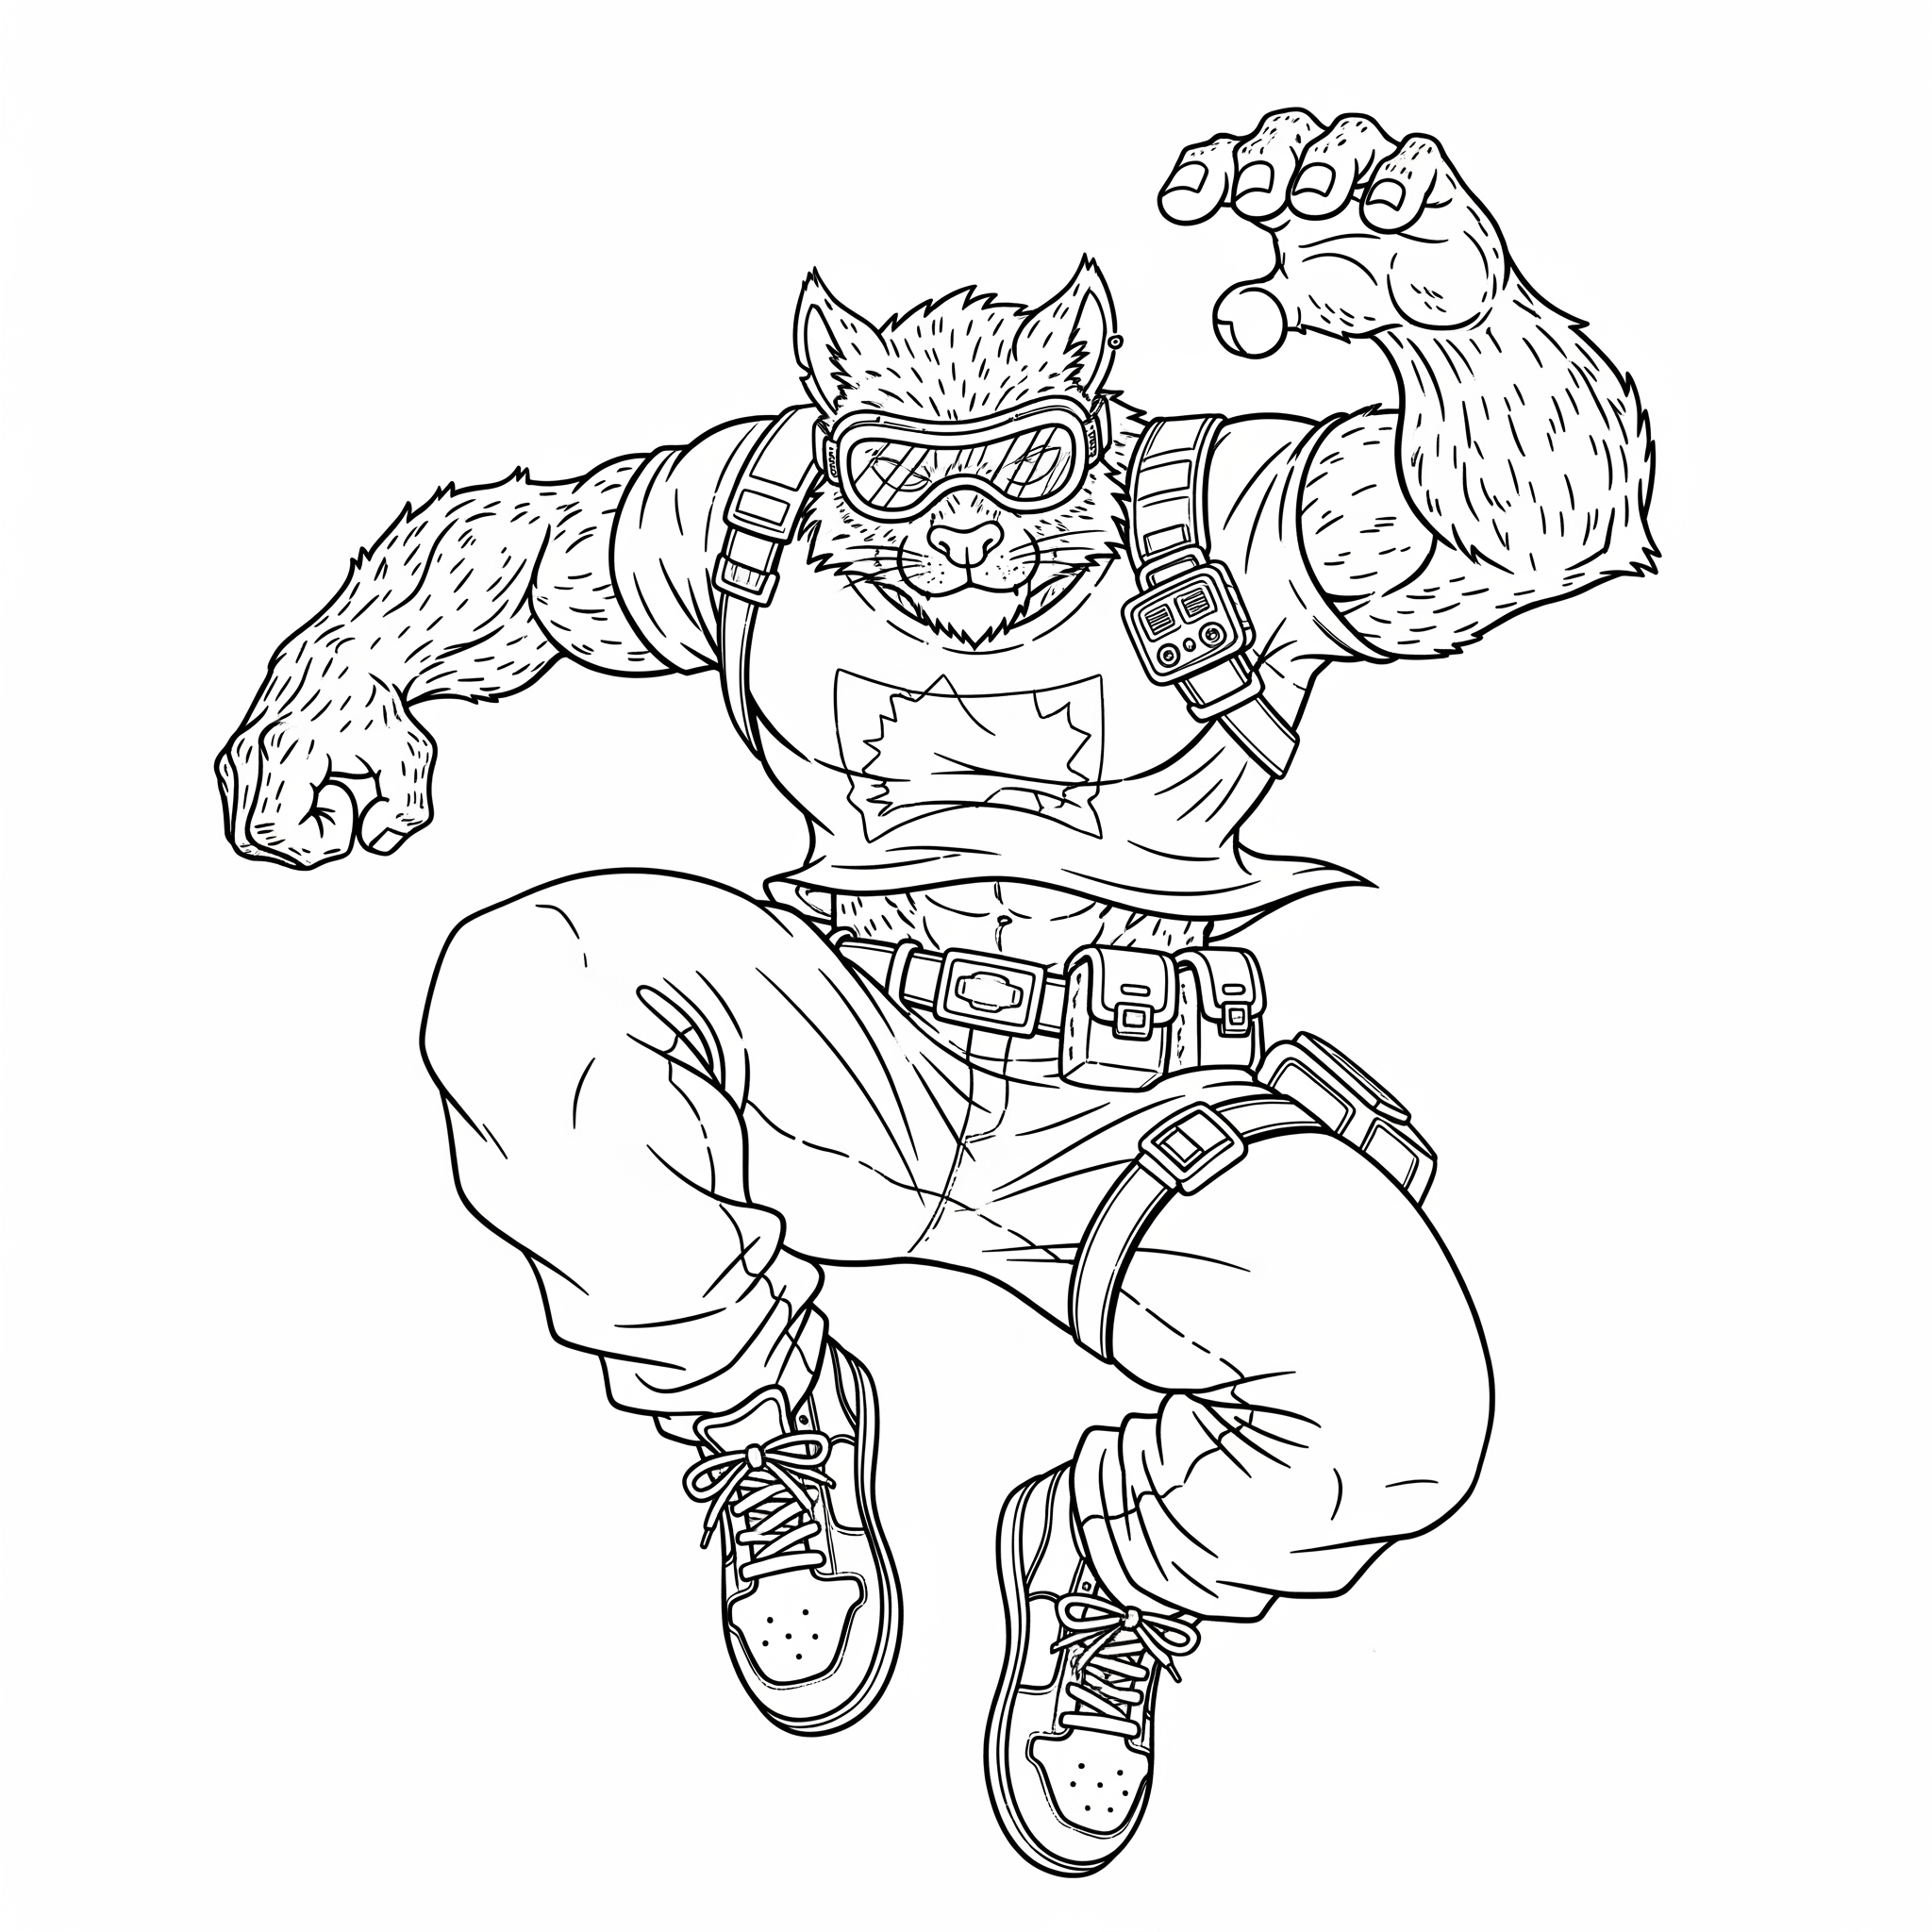
\includegraphics[width=12cm]{images/frontCover.png}
\end{figure}
\centering\Huge\fontspec{TradeWinds-Regular.ttf}Martial Mutant Misfitz!

\newpage
\pagenumbering{arabic}

\section*{\fontspec{TradeWinds-Regular.ttf}What is Martial Mutant Misfitz?}
\raggedright\normalfont\large You are humanoid animal mutants. Human society rejects you. Your appearance is alien and off-putting to most humans. Fortunately, a mentor came into your life. Taking care of you when you needed it the most. Training you in martial prowess, and teaching you how to leverage your new abilities. A mentor hiding your from society and shielding you from harm. But this could soon end, as a new evil rises, that threatens the city. Who is gonna stop it? Who if not you?!

Martial Mutant Misfitz is a game about whacky teenagers mutated into animals. It's a game about stylish fighting and kung fu. It also is a game about being an outsider --- he feeling of not fitting into society. And lastly, it's a game about family.
\newpage

\renewcommand{\playbookTitle}{Brawler}

\renewcommand{\playbookImage}{images/brawler.png}

\renewcommand{\flavorText}{
\textit{Big muscles, bigger attitude. Always ready to rumble.}\\
\medskip
You love fighting and your mutations gave you the tools to really excel at it. This gives you the power to protect others. However, your hot headedness brings you a lot of trouble.\\
\medskip
Towards the others you always argue for acting. Too much diskussion gives you headaches.
}

\renewcommand{\charNames}{1.Knuckles, 2.Jax, 3.Brock, 4.Roxy, 5.Bruiza, 6.Wrecka, \rule{2cm}{1pt}}

\renewcommand{\charAnimals}{1.Bear, 2.Rhino, 3.Buffalo, 4.Crocodile, 5.Kangaroo, 6.Pangolin, \rule{2cm}{1pt}}

\renewcommand{\charEnhancementOne}{\textbf{Electrified Brass Knuckles} (2 harm, 1 harm ignores armor electric, 1 harm blunt hand)}
\renewcommand{\charEnhancementTwo}{\textbf{Spiked Wrist Wraps} (1 harm, quick, hand, blunt, pierce)}
\renewcommand{\charEnhancementThree}{\textbf{Tech-Spine} (makes all weapons quick)}
\renewcommand{\charEnhancementFour}{\textbf{Hardened Skin} (2 armor vs. piercing)}
\renewcommand{\charEnhancementFive}{\textbf{Razor Claws} (2 harm, hand, slash, pierce)}
\renewcommand{\charEnhancementSix}{\textbf{Steel Bones}  (2 armor vs. blunt)}

\renewcommand{\moveOne}{\textbf{One more word and I break your nose} If you try to provoke or intimidate someone you can roll +Grit on Talk the Talk}
\renewcommand{\moveTwo}{\textbf{Nothin' But a Scratch} Once per session you can roll +Discipline. On a 10+ heal 2 harm and stabilize your wounds. On a 7-9 you may stabilize or heal 1 harm. On a miss, it was worse than it looked}
\renewcommand{\moveThree}{\textbf{Walls are optional} When your break through walls, destroy or throw obstacles. Roll +Grit. On a hit, choose one of the following:
\vspace{-6pt}
\begin{itemize}
    \setlength\itemsep{-0.5em}
\item Deal 2 harm
\item Get or give +1 forward
\item You draw attention - enemies focus on you.
\item You create a advantageous position for your team.
\end{itemize}
\vspace{-6pt}
On a 7-9 additionally choose one of the following:
\vspace{-6pt}
\begin{itemize}
    \setlength\itemsep{-0.5em}
\item  Take 1 harm
\item  Take 1 condition
\end{itemize}

}
\renewcommand{\moveFour}{\textbf{Coming through!} When you charge at the enemy, you shrug off harm until your momentum stops.}
\renewcommand{\moveFive}{\textbf{You brought a gang? Cute.} Once per session, you can add area to any attack.}

\renewcommand{\relationsOne}{\rule{2cm}{1pt}'s and your fighting style derived from the same base style. How is it called? What does it look like? What is it about?}
\renewcommand{\relationsTwo}{You often get into trouble with \rule{2cm}{1pt}. Doing what?}
\renewcommand{\relationsThree}{When you were younger, \rule{2cm}{1pt} and you wrestled all the time. What famous wrestler did you embody?}

\renewcommand{\leadingPrinciplesOne}{Protect others}
\renewcommand{\leadingPrinciplesTwo}{Take action}
\renewcommand{\leadingPrinciplesThree}{Go solo}
\renewcommand{\leadingPrinciplesFour}{Take an ego trip}

\renewcommand{\flipsideOne}{Risk too much}
\renewcommand{\flipsideTwo}{Be impatient}
\renewcommand{\flipsideThree}{Freak out way too soon}
\renewcommand{\flipsideFour}{Think too little about a plan or problem}

\pagenumbering{gobble}

\vspace*{\fill}

\begin{figure}[h!]
\centering\includegraphics[width=12cm]{\playbookImage}
\vspace{-\baselineskip}\vspace{+0.1pt}
\rule{\linewidth}{2pt}
\end{figure}
\Huge\fontspec{TradeWinds-Regular.ttf}The \playbookTitle

\normalfont\large
\medskip

\flavorText

\newpage

\Large\fontspec{TradeWinds-Regular.ttf}Animal

\medskip

\normalfont\large \charAnimals

\medskip

\Large\fontspec{TradeWinds-Regular.ttf}Names

\medskip

\normalfont\large \charNames

\medskip

\Large\fontspec{TradeWinds-Regular.ttf}Enhancements

\medskip

\normalfont\large Pick or roll two:

\(\square\) \charEnhancementOne

\(\square\) \charEnhancementTwo

\(\square\) \charEnhancementThree

\(\square\) \charEnhancementFour

\(\square\) \charEnhancementFive

\(\square\) \charEnhancementSix

\medskip

\Large\fontspec{TradeWinds-Regular.ttf}Advancements \(\LARGE \Circle \Circle \Circle \Circle \Circle \)

\medskip

\normalfont\large

\begin{tabular}{l @{\hspace{2cm}} l}
\(\square\) Get +1 Power, max +3 & \(\square\) Take another \playbookTitle~move \\
\(\square\) Get +1 Cool, max +3 & \(\square\) Take another \playbookTitle~enhancement \\
\(\square\) Get +1 Wits, max +3 & \(\square\) Take a move from another playbook \\
\(\square\) Get +1 Heart, max +3 & \(\square\) Take a move from another playbook \\
\(\square\) Get +1 Weird, max +3 & \\
\end{tabular}

\medskip

\Large\fontspec{TradeWinds-Regular.ttf}Conditions

\medskip

\normalfont\large

\(\square\) \textbf{Exposed} (-2 to Power until you eliminate or evade the skeptical)\\
\(\square\) \textbf{Angry} (-2 to Cool until you hurt someone or break something)\\
\(\square\) \textbf{Stressed} (-2 to Weird until you say sth hurtful to someone)\\
\(\square\) \textbf{Jealous} (-2 to Heart until you go on an ego trip)\\
\(\square\) \textbf{Insecure} (-2 to Charm until you take a comment to wrong way)\\
\(\square\) \textbf{Poisoned}  (-1 to all stats until healed)

\medskip

\Large\fontspec{TradeWinds-Regular.ttf}Harm \(\bigtriangledown \bigtriangledown \bigtriangledown \bigtriangledown | \bigtriangledown \bigtriangledown\)

\medskip

\Large\fontspec{TradeWinds-Regular.ttf}Stats

\normalfont\Huge

%Add tabular?
\faBomb~\textcolor{lightgray}{\faCircle[regular]} \hspace{0.5cm} \faStar~\textcolor{lightgray}{\faCircle[regular]} \hspace{0.5cm} \faHeart~\textcolor{lightgray}{\faCircle[regular]} \hspace{0.5cm} \faBrain~\textcolor{lightgray}{\faCircle[regular]} \hspace{0.5cm} \faPizzaSlice~\textcolor{lightgray}{\faCircle[regular]}

\medskip

\Large\fontspec{TradeWinds-Regular.ttf}Notes

\newpage

\Large\fontspec{TradeWinds-Regular.ttf}\playbookTitle~Moves

\medskip

\normalfont\large

\begin{itemize}[label=$\square$]

\item \moveOne

\item \moveTwo

\item \moveThree

\item \moveFour

\item \moveFive

\end{itemize}


\Large\fontspec{TradeWinds-Regular.ttf}Relations

\medskip

\normalfont\large

\begin{itemize}[label=$\square$]
    \item \relationsOne
    \item \relationsTwo
    \item \relationsThree
\end{itemize}

\begin{tabular}{l @{\hspace{2cm}} l}

\Large\fontspec{TradeWinds-Regular.ttf}Leading Principles & \Large\fontspec{TradeWinds-Regular.ttf}Flipside \\

\normalfont\large

$\bullet$ \leadingPrinciplesOne & $\bullet$ \flipsideOne \\
$\bullet$ \leadingPrinciplesTwo &  $\bullet$ \flipsideTwo \\
$\bullet$ \leadingPrinciplesThree &  $\bullet$ \flipsideThree \\
$\bullet$ \leadingPrinciplesFour &  $\bullet$ \flipsideFour \\

\end{tabular}

\newpage
\renewcommand{\playbookTitle}{Brainiac}

\renewcommand{\playbookImage}{images/brainiac.png}

\renewcommand{\flavorText}{
\textit{"For every problem there is a solution and I will find it."}\\
\medskip
You love science and solving puzzles. You are the brains of your team.\\
\medskip
Towards the others you often pled for waiting to receive more data, diskussing and analyzing.
}

\renewcommand{\charNames}{1.Cypher, 2.Echo, 3.Vector, 4.Ivy, 5.Pixel, 6.Glitch, \rule{2cm}{1pt}}

\renewcommand{\charAnimals}{1.Octopus, 2.Raven, 3.Owl, 4.Dolphin, 5.Fox, 6.Gorilla, \rule{2cm}{1pt}}

\renewcommand{\charEnhancementOne}{\textbf{MutaTech Mark IV Attack Drones} (1 harm, far)}
\renewcommand{\charEnhancementTwo}{\textbf{Backpack-Lab} Gives you the opportunity to analyze and synthesize chemicals on the go.}
\renewcommand{\charEnhancementThree}{\textbf{MorphSwarm Units} (1 harm, hand, choose blunt, piercing, …)}
\renewcommand{\charEnhancementFour}{\textbf{Hyper-Cognition} (choose one additional move)}
\renewcommand{\charEnhancementFive}{\textbf{Ultra-Adaptive NeuroShield} (1 armor)}
\renewcommand{\charEnhancementSix}{\textbf{EMP} (1 harm vs. mechanical, area)}

\renewcommand{\moveOne}{\textbf{This won’t take long.} Hack, repair or manipulate something. Roll +Wits. On a hit you surpass the challenge. On a 7-9 you only get a limited time in the system.}
\renewcommand{\moveTwo}{
You can’t hide from thermals. Roll +Wits. On a 10+, ask the GM two of the following questions, on a 7-9 one.
\begin{itemize}
    \item Is there someone behind this wall?
    \item What would someone see if the visibility was better?
    \item How many individuals are we dealing with?
    \item What is a weak spot here?
    \item How do we get in or out?
    \item What is the safest way forward?
    \item What is some valuable piece of information?
\end{itemize}
}
\renewcommand{\moveThree}{\textbf{Hope they backed this up.} When you receive information or hack into a system, you get or give +1 forward.}
\renewcommand{\moveFour}{\textbf{Crafted with love... and a little bit of panic.} Roll +Weird. On a hit you improvise a weapon (1 harm) and get +1 forward. On a 7-9 it only lasts for this combat.}
\renewcommand{\moveFive}{\textbf{Keep calm and pretend this is fine.} Roll +Weird. On a hit you clear a condition off of you}

\renewcommand{\relationsOne}{\rule{2cm}{1pt} and I love the same video game. How is it called? What is it about?}
\renewcommand{\relationsTwo}{I taught \rule{2cm}{1pt} about the science field I love. What is it?}
\renewcommand{\relationsThree}{I found unusual data or browser history from \rule{2cm}{1pt} on the shared computer. Ask the player what it was about.}

\renewcommand{\leadingPrinciplesOne}{Be the rationale}
\renewcommand{\leadingPrinciplesTwo}{Solve puzzles}
\renewcommand{\leadingPrinciplesThree}{Provide information}
\renewcommand{\leadingPrinciplesFour}{Correct wrong or imprecise information}

\renewcommand{\flipsideOne}{Think too long}
\renewcommand{\flipsideTwo}{Don't act}
\renewcommand{\flipsideThree}{Be hesitant}
\renewcommand{\flipsideFour}{Have troubles deciding}

\pagenumbering{gobble}

\vspace*{\fill}

\begin{figure}[h!]
\centering\includegraphics[width=12cm]{\playbookImage}
\vspace{-\baselineskip}\vspace{+0.1pt}
\rule{\linewidth}{2pt}
\end{figure}
\Huge\fontspec{TradeWinds-Regular.ttf}The \playbookTitle

\normalfont\large
\medskip

\flavorText

\newpage

\Large\fontspec{TradeWinds-Regular.ttf}Animal

\medskip

\normalfont\large \charAnimals

\medskip

\Large\fontspec{TradeWinds-Regular.ttf}Names

\medskip

\normalfont\large \charNames

\medskip

\Large\fontspec{TradeWinds-Regular.ttf}Enhancements

\medskip

\normalfont\large Pick or roll two:

\(\square\) \charEnhancementOne

\(\square\) \charEnhancementTwo

\(\square\) \charEnhancementThree

\(\square\) \charEnhancementFour

\(\square\) \charEnhancementFive

\(\square\) \charEnhancementSix

\medskip

\Large\fontspec{TradeWinds-Regular.ttf}Advancements \(\LARGE \Circle \Circle \Circle \Circle \Circle \)

\medskip

\normalfont\large

\begin{tabular}{l @{\hspace{2cm}} l}
\(\square\) Get +1 Power, max +3 & \(\square\) Take another \playbookTitle~move \\
\(\square\) Get +1 Cool, max +3 & \(\square\) Take another \playbookTitle~enhancement \\
\(\square\) Get +1 Wits, max +3 & \(\square\) Take a move from another playbook \\
\(\square\) Get +1 Heart, max +3 & \(\square\) Take a move from another playbook \\
\(\square\) Get +1 Weird, max +3 & \\
\end{tabular}

\medskip

\Large\fontspec{TradeWinds-Regular.ttf}Conditions

\medskip

\normalfont\large

\(\square\) \textbf{Exposed} (-2 to Power until you eliminate or evade the skeptical)\\
\(\square\) \textbf{Angry} (-2 to Cool until you hurt someone or break something)\\
\(\square\) \textbf{Stressed} (-2 to Weird until you say sth hurtful to someone)\\
\(\square\) \textbf{Jealous} (-2 to Heart until you go on an ego trip)\\
\(\square\) \textbf{Insecure} (-2 to Charm until you take a comment to wrong way)\\
\(\square\) \textbf{Poisoned}  (-1 to all stats until healed)

\medskip

\Large\fontspec{TradeWinds-Regular.ttf}Harm \(\bigtriangledown \bigtriangledown \bigtriangledown \bigtriangledown | \bigtriangledown \bigtriangledown\)

\medskip

\Large\fontspec{TradeWinds-Regular.ttf}Stats

\normalfont\Huge

%Add tabular?
\faBomb~\textcolor{lightgray}{\faCircle[regular]} \hspace{0.5cm} \faStar~\textcolor{lightgray}{\faCircle[regular]} \hspace{0.5cm} \faHeart~\textcolor{lightgray}{\faCircle[regular]} \hspace{0.5cm} \faBrain~\textcolor{lightgray}{\faCircle[regular]} \hspace{0.5cm} \faPizzaSlice~\textcolor{lightgray}{\faCircle[regular]}

\medskip

\Large\fontspec{TradeWinds-Regular.ttf}Notes

\newpage

\Large\fontspec{TradeWinds-Regular.ttf}\playbookTitle~Moves

\medskip

\normalfont\large

\begin{itemize}[label=$\square$]

\item \moveOne

\item \moveTwo

\item \moveThree

\item \moveFour

\item \moveFive

\end{itemize}


\Large\fontspec{TradeWinds-Regular.ttf}Relations

\medskip

\normalfont\large

\begin{itemize}[label=$\square$]
    \item \relationsOne
    \item \relationsTwo
    \item \relationsThree
\end{itemize}

\begin{tabular}{l @{\hspace{2cm}} l}

\Large\fontspec{TradeWinds-Regular.ttf}Leading Principles & \Large\fontspec{TradeWinds-Regular.ttf}Flipside \\

\normalfont\large

$\bullet$ \leadingPrinciplesOne & $\bullet$ \flipsideOne \\
$\bullet$ \leadingPrinciplesTwo &  $\bullet$ \flipsideTwo \\
$\bullet$ \leadingPrinciplesThree &  $\bullet$ \flipsideThree \\
$\bullet$ \leadingPrinciplesFour &  $\bullet$ \flipsideFour \\

\end{tabular}

\newpage
\renewcommand{\playbookTitle}{Wildcard}

\renewcommand{\playbookImage}{images/wildcard.png}

\renewcommand{\flavorText}{
Fast-talking, fast-riding, always radical. Every deck needs a wild card.\\
\medskip
You are chaotic, stylish and emotional. If you don't feel it, it's not happening. You do what you love and you do it with style.
}

\renewcommand{\charNames}{1.Sparx, 2.Jinx, 3.Blitz, 4.Fizz, 5.Zeke, 6.Turbo, \rule{2cm}{1pt}}

\renewcommand{\charAnimals}{1.Platypus, 2.Sloth, 3.Otter, 4.Gecko, 5.Red Panda, 6.Anteater, \rule{2cm}{1pt}}

\renewcommand{\charEnhancementOne}{\textbf{Molotow Graffiti Cans} (1 harm, area, close)}
\renewcommand{\charEnhancementTwo}{\textbf{Skateboard} (+1 on Ride or Slide)}
\renewcommand{\charEnhancementThree}{\textbf{Razorwire BladeYoyo} (2 harm, close)}
\renewcommand{\charEnhancementFour}{\textbf{Lucky coin} (once per session, reroll)}
\renewcommand{\charEnhancementFive}{\textbf{Hyperflex Skeleton} (no falling damage)}
\renewcommand{\charEnhancementSix}{\textbf{Sprayer Mask} (immune to gaseous toxins)}

\renewcommand{\moveOne}{\textbf{I'm just a veeery weird cosplayer.} Get +1 when trying to Blend In}
\renewcommand{\moveTwo}{
\textbf{10\% skill, 90\% bad decisions!} Whenever you do some form of stunt, roll +Cool. On a hit choose one of the following
\begin{itemize}
    \item Get somewhere no-one else can
    \item Get +1 forward
    \item Impress or distract
    \item Create a new route or shortcut
\end{itemize}
On a 7-9 additionally choose one of the following
\begin{itemize}
    \item Get 1 harm
    \item Get a condition
    \item Draw unwanted attention
    \item You're off-balance or vulnerable for a moment
\end{itemize}
}
\renewcommand{\moveThree}{\textbf{Art school's overrated.} You can get information from graffitis. You can tag to influence other sprayers. Orientation in the city is therefore enhanced.}
\renewcommand{\moveFour}{\textbf{Style points? Maxed out.} You weave style and tricks into your fighting and become unpredictable. When you Kick Shell! you can roll +Weird.}
\renewcommand{\moveFive}{\textbf{I licked it already. You're welcome.} You always have some form of junk food with you. When you offer it to someone, they roll +Weird. One a hit, they remove 1 harm, on a 7-9 they get a condition.}

\renewcommand{\relationsOne}{You and \rule{2cm}{1pt} obsess over the same junk food. What is it?}
\renewcommand{\relationsTwo}{\rule{2cm}{1pt} found your art and was surprised by it. What did you draw?}
\renewcommand{\relationsThree}{You taught \rule{2cm}{1pt} some tricks. In what sport and what tricks?}

\renewcommand{\leadingPrinciplesOne}{Be chaotic}
\renewcommand{\leadingPrinciplesTwo}{Think outside the box}
\renewcommand{\leadingPrinciplesThree}{Live in the moment}
\renewcommand{\leadingPrinciplesFour}{Have passion}

\renewcommand{\flipsideOne}{Seek crazy experiences}
\renewcommand{\flipsideTwo}{Get addicted to something}
\renewcommand{\flipsideThree}{Avoid being bored at all cost}
\renewcommand{\flipsideFour}{Put yourself or others in danger}

\pagenumbering{gobble}

\vspace*{\fill}

\begin{figure}[h!]
\centering\includegraphics[width=12cm]{\playbookImage}
\vspace{-\baselineskip}\vspace{+0.1pt}
\rule{\linewidth}{2pt}
\end{figure}
\Huge\fontspec{TradeWinds-Regular.ttf}The \playbookTitle

\normalfont\large
\medskip

\flavorText

\newpage

\Large\fontspec{TradeWinds-Regular.ttf}Animal

\medskip

\normalfont\large \charAnimals

\medskip

\Large\fontspec{TradeWinds-Regular.ttf}Names

\medskip

\normalfont\large \charNames

\medskip

\Large\fontspec{TradeWinds-Regular.ttf}Enhancements

\medskip

\normalfont\large Pick or roll two:

\(\square\) \charEnhancementOne

\(\square\) \charEnhancementTwo

\(\square\) \charEnhancementThree

\(\square\) \charEnhancementFour

\(\square\) \charEnhancementFive

\(\square\) \charEnhancementSix

\medskip

\Large\fontspec{TradeWinds-Regular.ttf}Advancements \(\LARGE \Circle \Circle \Circle \Circle \Circle \)

\medskip

\normalfont\large

\begin{tabular}{l @{\hspace{2cm}} l}
\(\square\) Get +1 Power, max +3 & \(\square\) Take another \playbookTitle~move \\
\(\square\) Get +1 Cool, max +3 & \(\square\) Take another \playbookTitle~enhancement \\
\(\square\) Get +1 Wits, max +3 & \(\square\) Take a move from another playbook \\
\(\square\) Get +1 Heart, max +3 & \(\square\) Take a move from another playbook \\
\(\square\) Get +1 Weird, max +3 & \\
\end{tabular}

\medskip

\Large\fontspec{TradeWinds-Regular.ttf}Conditions

\medskip

\normalfont\large

\(\square\) \textbf{Exposed} (-2 to Power until you eliminate or evade the skeptical)\\
\(\square\) \textbf{Angry} (-2 to Cool until you hurt someone or break something)\\
\(\square\) \textbf{Stressed} (-2 to Weird until you say sth hurtful to someone)\\
\(\square\) \textbf{Jealous} (-2 to Heart until you go on an ego trip)\\
\(\square\) \textbf{Insecure} (-2 to Charm until you take a comment to wrong way)\\
\(\square\) \textbf{Poisoned}  (-1 to all stats until healed)

\medskip

\Large\fontspec{TradeWinds-Regular.ttf}Harm \(\bigtriangledown \bigtriangledown \bigtriangledown \bigtriangledown | \bigtriangledown \bigtriangledown\)

\medskip

\Large\fontspec{TradeWinds-Regular.ttf}Stats

\normalfont\Huge

%Add tabular?
\faBomb~\textcolor{lightgray}{\faCircle[regular]} \hspace{0.5cm} \faStar~\textcolor{lightgray}{\faCircle[regular]} \hspace{0.5cm} \faHeart~\textcolor{lightgray}{\faCircle[regular]} \hspace{0.5cm} \faBrain~\textcolor{lightgray}{\faCircle[regular]} \hspace{0.5cm} \faPizzaSlice~\textcolor{lightgray}{\faCircle[regular]}

\medskip

\Large\fontspec{TradeWinds-Regular.ttf}Notes

\newpage

\Large\fontspec{TradeWinds-Regular.ttf}\playbookTitle~Moves

\medskip

\normalfont\large

\begin{itemize}[label=$\square$]

\item \moveOne

\item \moveTwo

\item \moveThree

\item \moveFour

\item \moveFive

\end{itemize}


\Large\fontspec{TradeWinds-Regular.ttf}Relations

\medskip

\normalfont\large

\begin{itemize}[label=$\square$]
    \item \relationsOne
    \item \relationsTwo
    \item \relationsThree
\end{itemize}

\begin{tabular}{l @{\hspace{2cm}} l}

\Large\fontspec{TradeWinds-Regular.ttf}Leading Principles & \Large\fontspec{TradeWinds-Regular.ttf}Flipside \\

\normalfont\large

$\bullet$ \leadingPrinciplesOne & $\bullet$ \flipsideOne \\
$\bullet$ \leadingPrinciplesTwo &  $\bullet$ \flipsideTwo \\
$\bullet$ \leadingPrinciplesThree &  $\bullet$ \flipsideThree \\
$\bullet$ \leadingPrinciplesFour &  $\bullet$ \flipsideFour \\

\end{tabular}

\newpage
\renewcommand{\playbookTitle}{Leader}

\renewcommand{\playbookImage}{images/leader.png}

\renewcommand{\flavorText}{
\textit{The team is the most important. To me, you are my family.}\\
\medskip
You coordinate and bring the team together. You try to hear every voice in the team and try to compromise. In the field you often try to coordinate this chaotic crew of mutants.
}

\renewcommand{\charNames}{1.Rex, 2.Scar, 3.Cinder, 4.Ash, 5.Vax, 6.Crash, \rule{2cm}{1pt}}

\renewcommand{\charAnimals}{1.Turtle, 2.Rhino, 3.Bear, 4.Lion, 5.Falcon, 6.Mustang \rule{2cm}{1pt}}

\renewcommand{\charEnhancementOne}{\textbf{Kinetic Shield} (1 armor)}
\renewcommand{\charEnhancementTwo}{\textbf{Magnetron Core} (+1 on Ride or Slide)}
\renewcommand{\charEnhancementThree}{\textbf{Warcry} (+1 to \emph{Team-Up!})}
\renewcommand{\charEnhancementFour}{\textbf{Ancient Katana from your Mentor} (2 harm, hand, slash, pierce)}
\renewcommand{\charEnhancementFive}{\textbf{MutaTech Vibro Polearm} (1 harm, close, slash, pierce)}
\renewcommand{\charEnhancementSix}{\textbf{Tactical HUD} (Always know the condition of team mates)}

\renewcommand{\moveOne}{\textbf{Keep tight, hit hard} When you coordinate the team, roll +Discipline. On a hit you raise the Team Mojo by 1. On a 10+ you additionally get +1 forward.}
\renewcommand{\moveTwo}{\textbf{Semper paratis} whenever your fall back on your preperations, roll +Style. On a 10+ you have just the thing. On a 7-9 you do not have the perfect solution, but something close, ask the GM what.}
\renewcommand{\moveThree}{\textbf{I see the play.} Whenever you read a tactical situation roll +Discipline. On a hit, ask the GM one question, on a 10+ two.
\vspace{-6pt}
\begin{itemize}
    \setlength\itemsep{-0.5em}
    \item Where is a weak spot?
    \item What's the biggest threat?
    \item Who is out of position?
    \item What is there to do to end this fast?
\end{itemize}
}
\renewcommand{\moveFour}{\textbf{Not on my watch.} Once per scene, you can take the harm or condition of others.}
\renewcommand{\moveFive}{\textbf{I've seen this before.} Once per session, you can declare how you trained for this exact scenario and gain +1 forward.}

\renewcommand{\relationsOne}{\rule{2cm}{1pt} saw you fail. In what situation?}
\renewcommand{\relationsTwo}{You took the fall for \rule{2cm}{1pt}. Ask the player for what.}
\renewcommand{\relationsThree}{\rule{2cm}{1pt} made a mixtape. You hate 90\% of it. You never turn it off. Ask the player what music is on it.}

\renewcommand{\leadingPrinciplesOne}{Hear everyone out}
\renewcommand{\leadingPrinciplesTwo}{Moderate a discussion}
\renewcommand{\leadingPrinciplesThree}{Decide}
\renewcommand{\leadingPrinciplesFour}{Find compromises}

\renewcommand{\flipsideOne}{Feel helpless}
\renewcommand{\flipsideTwo}{Compromises are not always the best for everyone}
\renewcommand{\flipsideThree}{You come too short}
\renewcommand{\flipsideFour}{You chose the wrong course of action}

\pagenumbering{gobble}

\vspace*{\fill}

\begin{figure}[h!]
\centering\includegraphics[width=12cm]{\playbookImage}
\vspace{-\baselineskip}\vspace{+0.1pt}
\rule{\linewidth}{2pt}
\end{figure}
\Huge\fontspec{TradeWinds-Regular.ttf}The \playbookTitle

\normalfont\large
\medskip

\flavorText

\newpage

\Large\fontspec{TradeWinds-Regular.ttf}Animal

\medskip

\normalfont\large \charAnimals

\medskip

\Large\fontspec{TradeWinds-Regular.ttf}Names

\medskip

\normalfont\large \charNames

\medskip

\Large\fontspec{TradeWinds-Regular.ttf}Enhancements

\medskip

\normalfont\large Pick or roll two:

\(\square\) \charEnhancementOne

\(\square\) \charEnhancementTwo

\(\square\) \charEnhancementThree

\(\square\) \charEnhancementFour

\(\square\) \charEnhancementFive

\(\square\) \charEnhancementSix

\medskip

\Large\fontspec{TradeWinds-Regular.ttf}Advancements \(\LARGE \Circle \Circle \Circle \Circle \Circle \)

\medskip

\normalfont\large

\begin{tabular}{l @{\hspace{2cm}} l}
\(\square\) Get +1 Power, max +3 & \(\square\) Take another \playbookTitle~move \\
\(\square\) Get +1 Cool, max +3 & \(\square\) Take another \playbookTitle~enhancement \\
\(\square\) Get +1 Wits, max +3 & \(\square\) Take a move from another playbook \\
\(\square\) Get +1 Heart, max +3 & \(\square\) Take a move from another playbook \\
\(\square\) Get +1 Weird, max +3 & \\
\end{tabular}

\medskip

\Large\fontspec{TradeWinds-Regular.ttf}Conditions

\medskip

\normalfont\large

\(\square\) \textbf{Exposed} (-2 to Power until you eliminate or evade the skeptical)\\
\(\square\) \textbf{Angry} (-2 to Cool until you hurt someone or break something)\\
\(\square\) \textbf{Stressed} (-2 to Weird until you say sth hurtful to someone)\\
\(\square\) \textbf{Jealous} (-2 to Heart until you go on an ego trip)\\
\(\square\) \textbf{Insecure} (-2 to Charm until you take a comment to wrong way)\\
\(\square\) \textbf{Poisoned}  (-1 to all stats until healed)

\medskip

\Large\fontspec{TradeWinds-Regular.ttf}Harm \(\bigtriangledown \bigtriangledown \bigtriangledown \bigtriangledown | \bigtriangledown \bigtriangledown\)

\medskip

\Large\fontspec{TradeWinds-Regular.ttf}Stats

\normalfont\Huge

%Add tabular?
\faBomb~\textcolor{lightgray}{\faCircle[regular]} \hspace{0.5cm} \faStar~\textcolor{lightgray}{\faCircle[regular]} \hspace{0.5cm} \faHeart~\textcolor{lightgray}{\faCircle[regular]} \hspace{0.5cm} \faBrain~\textcolor{lightgray}{\faCircle[regular]} \hspace{0.5cm} \faPizzaSlice~\textcolor{lightgray}{\faCircle[regular]}

\medskip

\Large\fontspec{TradeWinds-Regular.ttf}Notes

\newpage

\Large\fontspec{TradeWinds-Regular.ttf}\playbookTitle~Moves

\medskip

\normalfont\large

\begin{itemize}[label=$\square$]

\item \moveOne

\item \moveTwo

\item \moveThree

\item \moveFour

\item \moveFive

\end{itemize}


\Large\fontspec{TradeWinds-Regular.ttf}Relations

\medskip

\normalfont\large

\begin{itemize}[label=$\square$]
    \item \relationsOne
    \item \relationsTwo
    \item \relationsThree
\end{itemize}

\begin{tabular}{l @{\hspace{2cm}} l}

\Large\fontspec{TradeWinds-Regular.ttf}Leading Principles & \Large\fontspec{TradeWinds-Regular.ttf}Flipside \\

\normalfont\large

$\bullet$ \leadingPrinciplesOne & $\bullet$ \flipsideOne \\
$\bullet$ \leadingPrinciplesTwo &  $\bullet$ \flipsideTwo \\
$\bullet$ \leadingPrinciplesThree &  $\bullet$ \flipsideThree \\
$\bullet$ \leadingPrinciplesFour &  $\bullet$ \flipsideFour \\

\end{tabular}

\newpage

\end{document}